\documentclass[letterpaper,11pt]{article}

\usepackage{listings}
\usepackage{extarrows}
\usepackage{amssymb}
\usepackage{color}

\definecolor{dkgreen}{rgb}{0,0.6,0}
\definecolor{gray}{rgb}{0.5,0.5,0.5}
\definecolor{mauve}{rgb}{0.58,0,0.82}

\lstset{frame=tb,
  language=Python,
  aboveskip=3mm,
  belowskip=3mm,
  showstringspaces=false,
  columns=flexible,
  basicstyle={\small\ttfamily},
  numbers=none,
  numberstyle=\tiny\color{gray},
  keywordstyle=\color{blue},
  commentstyle=\color{dkgreen},
  stringstyle=\color{mauve},
  breaklines=true,
  breakatwhitespace=true,
  tabsize=3
}

\usepackage{setspace}
\usepackage{graphicx}
\usepackage{indentfirst}
\usepackage{bm}    %for textbf
\usepackage{amsmath}
\usepackage{amsfonts}   %for mathbb
\allowdisplaybreaks[4]  %from {amsmath}
\newcommand{\independent}{\rotatebox[origin=c]{90}{$\models$}}  %from {graphicx}
\usepackage{geometry}
\geometry{letterpaper, scale=0.8}  %from {geometry}
\author{Yuan Yin A20447290}
\title{MATH 588 Homework 3}
\begin{document}\large
\maketitle
\begin{spacing}{1.2}  %from {setspace}
\section*{Problem 1}

According to the last homework, we have pmf for $L$ and $L_1+L_2$ as follows:

\begin{table}[h]
\centering
\caption{pmf of L}
\begin{tabular}{|c|c|c|}
\hline
$L$ & $-50$ & $1000$\\
\hline
$\mathbb{P}$ & $p=0.991$ & $1-p = 0.009$\\
\hline
\end{tabular}
\end{table}

\begin{table}[h]
\centering
\caption{pmf of $L_1+L_2$}
\begin{tabular}{|c|c|c|c|}
\hline
$L^1+L^2$ & $-100$ & $950$ & $2000$\\
\hline
$\mathbb{P}$ & $0.991^2$ & $2*0.991*0.009$ & $0.009^2$\\
\hline
\end{tabular}
\end{table}

(a)
First we compute $Ent(L)$, since there is no restriction for $\alpha$, I plot value of $Ent(L)$ with varying $\alpha$ from 0 to 10. By Taylor, $Ent(L) = \frac{1}{\alpha}ln\mathbb{E}[e^{\alpha L}] \approx \mathbb{E}[L] + \frac{\alpha}{2} Var[L] + \sigma(\alpha^2)$. The code is in Appendix.

\begin{figure}[h]        
 \center{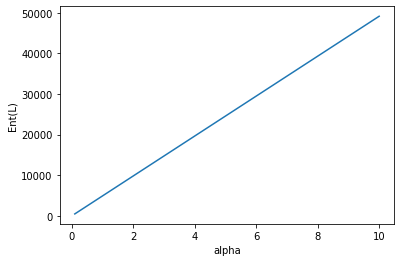
\includegraphics[scale=0.5]  {problem1a_Ent.png}}        
 \caption{\label{1} Ent(L)}      
 \end{figure}

Now we compute $SR(L):= -\frac{\mathbb{E}(L)}{Std(L)}$.

\begin{equation}
\begin{aligned}
SR(L) &= -\frac{\mathbb{E}(L)}{Std(L)} \\
&= -\frac{-50*0.991+1000*0.009}{\sqrt{Var(L)}} \\
&= -\frac{-40.55}{\sqrt{\mathbb{E}(L - \mathbb{E}(L))^2}} \\
&= -\frac{-40.55}{\sqrt{(-50+40.55)^2 * 0.991 + (1000+40.55)^2 * 0.009}} \\
&= 0.4089248259600986
\end{aligned}
\end{equation}

Then we compute $GLR(L):= \begin{cases} -\frac{\mathbb{E}(L)}{\mathbb{E}(L^+)}, & \mbox{if } \mathbb{E}(L) \le 0 \\ 0, & \mbox{otherwise} \end{cases}$

Since $\mathbb{E}(L) = -40.55 < 0$,

\begin{equation}
\begin{aligned}
GLR(L) &= -\frac{\mathbb{E}(L)}{\mathbb{E}(L^+)} \\
&= -\frac{-50*0.991+1000*0.009}{1000*0.009} \\
&= 4.5055555555555555
\end{aligned}
\end{equation}

Finally we compute $SOR(L):= \begin{cases} -\frac{\mathbb{E}(L)}{\sqrt{\mathbb{E}[(L^+)^2]}}, & \mbox{if } \mathbb{E}(L) \le 0 \\ 0, & \mbox{otherwise} \end{cases}$

Since $\mathbb{E}(L) = -40.55 < 0$,

\begin{equation}
\begin{aligned}
SOR(L) &= -\frac{\mathbb{E}(L)}{\sqrt{\mathbb{E}[(L^+)^2]}} \\
&= -\frac{-50*0.991+1000*0.009}{\sqrt{1000^2*0.009}} \\
&= 0.4274345303994259
\end{aligned}
\end{equation}

(b) Again, do the same for $L_1+L_2$.

First we compute $Ent(L_1+L_2)$. Similarly, The code is in Appendix. The plot is in next page.

\begin{figure}[htbp]        
 \center{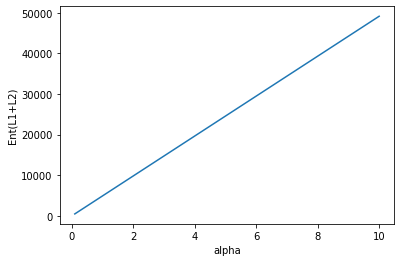
\includegraphics[scale=0.5]  {problem1b_Ent.png}}        
 \caption{\label{2} Ent($L_1+L_2$)}      
 \end{figure}


Now we compute $SR(L_1+L_2)$.

\begin{equation}
\begin{aligned}
SR(L_1+L_2) &= -\frac{\mathbb{E}(L_1+L_2)}{Std(L_1+L_2)} \\
&= -\frac{-100*0.991^2+950*2*0.991*0.009+2000*0.009^2}{\sqrt{Var(L_1+L_2)}} \\
&= -\frac{-81.1}{\sqrt{(-50+40.55)^2 * 0.991 + (1000+40.55)^2 * 0.009}} \\
&= 0.5783070348638291
\end{aligned}
\end{equation}

Then we compute $GLR(L_1+L_2)$

Since $\mathbb{E}(L_1+L_2) = -81.1 < 0$,

\begin{equation}
\begin{aligned}
GLR(L_1+L_2) &= -\frac{-81.1}{950*2*0.991*0.009+2000*0.009^2} \\
&= 4.740444584728871
\end{aligned}
\end{equation}

Finally we compute $SOR(L_1+L_2)$

Since $\mathbb{E}(L_1+L_2) = -81.1 < 0$,

\begin{equation}
\begin{aligned}
SOR(L_1+L_2) &= -\frac{\mathbb{E}(L)}{\sqrt{\mathbb{E}[(L^+)^2]}} \\
&= -\frac{-81.1}{\sqrt{950^2*2*0.991*0.009+2000^2*0.009^2}} \\
&= 0.6328449492330731
\end{aligned}
\end{equation}

(c)

Notice that if given value of correlation $\eta$, then we can compute $cov(L_1,L_2)$ by definition $\eta = \frac{cov(L_1,L_2)}{\sqrt{Var(L_1)Var(L_2)}}$, where $Var(L_1)$ and $Var(L_2)$ are known. We can slove the probability equation with the following table (next page):


\begin{table}[h]
\centering
\caption{pmf of $(L_1,L_2)$}
\begin{tabular}{|c|c|c|c|c|}
\hline
$(L_1,L_2)$ & $(-50,-50)$ & $(-50,1000)$ & $(1000,-50)$ & $(1000,1000)$\\
\hline
$\mathbb{P}$ & $a$ & $0.991-a$ & $0.991-a$ & $1-2*0.991+a$\\
\hline
\end{tabular}
\end{table}

where only ``$a$'' is unknown. This is because if we assume $\mathbb{P}\{(-50,-50)\} = a$, then $\mathbb{P}\{(-50,-50) \cup (-50,1000)\} = \mathbb{P}\{L_1 = -50\} = 0.991$. And similarly, $\mathbb{P}\{(-50,-50) \cup (1000,-50)\} = \mathbb{P}\{L_2 = -50\} = 0.991$. Therefore the table only have one unknown variable ``$a$''. And using $cov(L_1,L_2)$ we can compute $a$ easily.

I plot quantities in (a) with varying values of correlation, here I fix $\alpha=1$ when computing $Ent(L)$. Here is the plot (Code is in appendix):

\begin{figure}[htbp]        
 \center{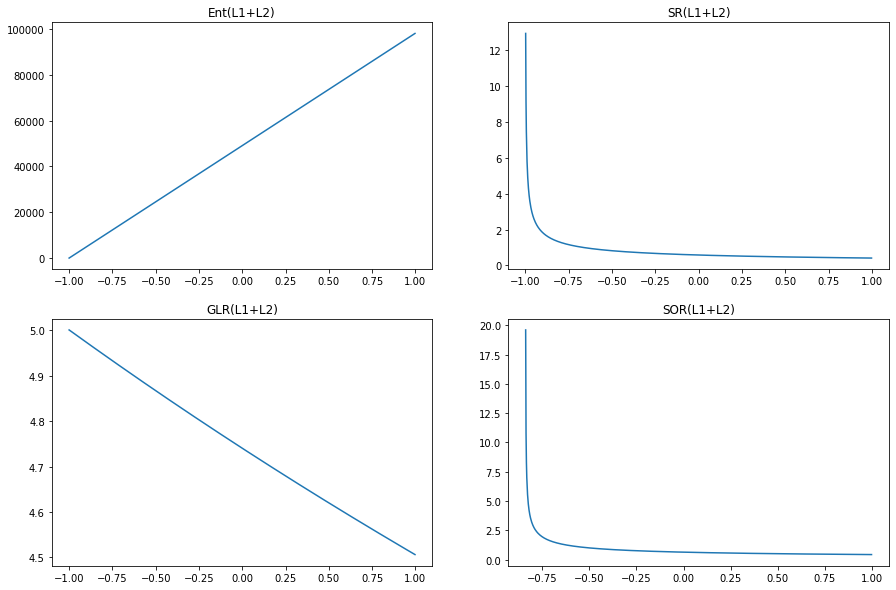
\includegraphics[scale=0.4]  {problem1c.png}}        
 \caption{\label{2} quantities for $L_1+L_2$ with correlation}      
 \end{figure}

\section*{Problem 2}
Knowing that $L_1 \sim \mathcal{N}(-1,1)$ and $L_2 = \max\{-1,L_1\}$. Thus, we can easily compute: $SR(L_1) = -\frac{\mathbb{E}(L_1)}{\sqrt{Var(L1)}} = 1$. Since by definition, $L_1 \le L_2$, to prove failure of monotone, we only need to show: $SR(L_2) \ge 1$.

It's easy to derive the cdf of $L_2$: $F_{L_2}(y):= 
\begin{cases} F_{L_1}(y), & \mbox{if } y \ge -1 \\
0, & \mbox{otherwise} \end{cases}$

Especially, the pdf is like: $\begin{cases} 
f_{L_1}(y), & \mbox{if } y > -1 \\
\frac{1}{2}, & \mbox{if } y = -1 \\
0, & \mbox{otherwise}
\end{cases}$

Thus,

\begin{equation}
\begin{aligned}
\mathbb{E}(L_2) &= (-1)*\frac{1}{2} + \int_{-1}^{\infty} x \frac{1}{\sqrt{2\pi}} e^{-\frac{(x+1)^2}{2}} dx = \frac{1}{\sqrt{2\pi}} - 1
\end{aligned}
\end{equation}

\begin{equation}
\begin{aligned}
\mathbb{E}(L_2^2) &= (-1)^2*\frac{1}{2} + \int_{-1}^{\infty} x^2 \frac{1}{\sqrt{2\pi}} e^{-\frac{(x+1)^2}{2}} dx\\
&\xlongequal{t:=x+1} \frac{1}{2} + \int_{0}^{\infty} (t-1)^2 \frac{1}{\sqrt{2\pi}} e^{-\frac{t^2}{2}} dt\\
&= \frac{1}{2} + \int_{0}^{\infty} t^2 \frac{1}{\sqrt{2\pi}} e^{-\frac{t^2}{2}} dt - 2\int_{0}^{\infty} t \frac{1}{\sqrt{2\pi}} e^{-\frac{t^2}{2}} dt + \int_{0}^{\infty} \frac{1}{\sqrt{2\pi}} e^{-\frac{t^2}{2}} dt\\
&= \frac{1}{2} + \frac{1}{2} + \frac{1}{2} - \frac{2}{\sqrt{2\pi}}
&= \frac{3}{2} - \frac{2}{\sqrt{2\pi}}
\end{aligned}
\end{equation}

Thus, $Var(L_2) = \frac{3}{2} - \frac{2}{\sqrt{2\pi}} - (\frac{1}{\sqrt{2\pi}} - 1)^2 = \frac{1}{2} - \frac{1}{2\pi} \Rightarrow SR(L_2) = -\frac{\mathbb{E}(L_2)}{\sqrt{Var(L2)}} \approx 1.0295 > 1$ 

Therefore, Sharpe ratio fails to be monotone for these two random variables.

\section*{Problem 3}

We need to prove $\alpha$ satisfies monotone, scale invariance and quasi-concave.

1. \textbf{Monotone: } $\forall L_1,L_2 \in \mathcal{M}, \mbox{if } L_1 \le L_2$, we need to show: $\alpha(L_1) \ge \alpha(L_2)$.

\textbf{proof: } Knowing that the probability set $(\mathcal{Q}^x)_{x \in [0,\infty]}$ is increasing, i.e. $\mathcal{Q}^x \subseteq \mathcal{Q}^y, \mbox{if } x \le y$.

Now, since $L_1 \le L_2$, for any fixed probability measure $\mathbb{Q}$, we have $\mathbb{E}_{\mathbb{Q}}[L_1] \le \mathbb{E}_{\mathbb{Q}}[L_2]$.

\begin{equation}
\begin{aligned}
&\Rightarrow \{\mathbb{E}_{\mathbb{Q}}[L_2] \le 0\} \Rightarrow \{\mathbb{E}_{\mathbb{Q}}[L_1] \le 0\} \\
&\Rightarrow \{\sup_{\mathbb{Q} \in \mathcal{Q}^x} \mathbb{E}_{\mathbb{Q}}[L_2] \le 0\} \Rightarrow \{\sup_{\mathbb{Q} \in \mathcal{Q}^x} \mathbb{E}_{\mathbb{Q}}[L_1] \le 0\} \ \mbox{(for some fixed x)}\\
&\Rightarrow \{\sup_{\mathbb{Q} \in \mathcal{Q}^x} \mathbb{E}_{\mathbb{Q}}[L_2] \le 0 \} \subseteq \{\sup_{\mathbb{Q} \in \mathcal{Q}^x} \mathbb{E}_{\mathbb{Q}}[L_1] \le 0 \} \ \mbox{(for some fixed x)}\\
&\Rightarrow \Big \{x \in [0,+\infty] | \sup_{\mathbb{Q} \in \mathcal{Q}^x} \mathbb{E}_{\mathbb{Q}}[L_2] \le 0 \Big \} \subseteq \Big \{ x \in [0,+\infty] | \sup_{\mathbb{Q} \in \mathcal{Q}^x} \mathbb{E}_{\mathbb{Q}}[L_1] \le 0 \Big \} \\
&\Rightarrow \sup \Big \{x \in [0,+\infty] | \sup_{\mathbb{Q} \in \mathcal{Q}^x} \mathbb{E}_{\mathbb{Q}}[L_2] \le 0 \Big \} \le \sup \Big \{ x \in [0,+\infty] | \sup_{\mathbb{Q} \in \mathcal{Q}^x} \mathbb{E}_{\mathbb{Q}}[L_1] \le 0 \Big \} \\
&\Rightarrow \alpha(L_2) \le \alpha(L_1) \quad \blacksquare
\end{aligned}
\end{equation}

2. \textbf{Scale invariance: } $\forall L \in \mathcal{M}, \lambda > 0$, we need to show: $\alpha(\lambda L) = \alpha(L)$.

\textbf{proof: } Since $\mathbb{E}[\lambda L] = \lambda \mathbb{E}[L]$, then for any fixed probability measure $\mathbb{Q}: $

\begin{equation}
\begin{aligned}
&\Rightarrow \mathbb{E}_{\mathbb{Q}}[\lambda L] \le 0 \Leftrightarrow \lambda \mathbb{E}_{\mathbb{Q}}[L] \le 0 \Leftrightarrow \mathbb{E}_{\mathbb{Q}}[L] \le 0, \ \mbox{for } \forall \lambda > 0 \\
&\Rightarrow \{\sup_{\mathbb{Q} \in \mathcal{Q}^x} \mathbb{E}_{\mathbb{Q}}[\lambda L] \le 0\} \Leftrightarrow \{\sup_{\mathbb{Q} \in \mathcal{Q}^x} \mathbb{E}_{\mathbb{Q}}[L] \le 0\}, \ \mbox{for } \forall \lambda > 0 \mbox{ and some fixed x} \\
&\Rightarrow \Big \{x \in [0,+\infty] | \sup_{\mathbb{Q} \in \mathcal{Q}^x} \mathbb{E}_{\mathbb{Q}}[\lambda L] \le 0 \Big \} \Leftrightarrow \Big \{ x \in [0,+\infty] | \sup_{\mathbb{Q} \in \mathcal{Q}^x} \mathbb{E}_{\mathbb{Q}}[L] \le 0 \Big \}, \ \mbox{for } \forall \lambda > 0 \\
&\Rightarrow \sup \Big \{x \in [0,+\infty] | \sup_{\mathbb{Q} \in \mathcal{Q}^x} \mathbb{E}_{\mathbb{Q}}[\lambda L] \le 0 \Big \} = \sup \Big \{ x \in [0,+\infty] | \sup_{\mathbb{Q} \in \mathcal{Q}^x} \mathbb{E}_{\mathbb{Q}}[L] \le 0 \Big \}, \ \mbox{for } \forall \lambda > 0 \\
&\Rightarrow \alpha(\lambda L) = \alpha(L), \ \mbox{for } \forall \lambda > 0 \quad \blacksquare
\end{aligned}
\end{equation}

3. \textbf{Quasi-concave: }$\forall L_1, L_2 \in \mathcal{M}, \lambda \in (0,1), m \in \mathbb{R}$, we need to show: if $\alpha(L_1) \ge m, \alpha(L_2) \ge m, \mbox{then } \alpha(\lambda L_1 + (1-\lambda) L_2) \ge m$.

\textbf{proof: } by property of scale invariant, we know $\alpha(L_1) = \alpha(\lambda L_1), \alpha(L_2) = \alpha((1-\lambda) L_2)$. Thus, $\alpha(\lambda L_1) \ge m, \alpha((1-\lambda) L_2) \ge m$. We have:

\begin{equation}
\begin{aligned}
&\Rightarrow \sup \Big \{x \in [0,+\infty] | \sup_{\mathbb{Q} \in \mathcal{Q}^x} \mathbb{E}_{\mathbb{Q}}[\lambda L_1] \le 0 \Big \} \ge \mbox{m}, \sup \Big \{ x \in [0,+\infty] | \sup_{\mathbb{Q} \in \mathcal{Q}^x} \mathbb{E}_{\mathbb{Q}}[(1-\lambda) L_2] \le 0 \Big \} \ge m \\
&\Rightarrow \sup_{\mathbb{Q} \in \mathcal{Q}^m} \mathbb{E}_{\mathbb{Q}}[\lambda L_1] \le 0, \sup_{\mathbb{Q} \in \mathcal{Q}^m} \mathbb{E}_{\mathbb{Q}}[(1-\lambda) L_2] \le 0 \\
&\Rightarrow \sup_{\mathbb{Q} \in \mathcal{Q}^m} \Big [ \mathbb{E}_{\mathbb{Q}}[\lambda L_1] + \mathbb{E}_{\mathbb{Q}}[(1-\lambda) L_2] \Big ] \le 0 \\
&\Rightarrow \sup_{\mathbb{Q} \in \mathcal{Q}^m} \mathbb{E}_{\mathbb{Q}}[\lambda L_1 + (1-\lambda) L_2] \le 0 \\
&\Rightarrow \sup \Big \{x \in [0,+\infty] | \sup_{\mathbb{Q} \in \mathcal{Q}^x} \mathbb{E}_{\mathbb{Q}}[\lambda L_1 + (1-\lambda) L_2] \le 0 \Big \} \ge \mbox{m} \\
&\Rightarrow \alpha(\lambda L_1 + (1-\lambda) L_2) \ge m \quad \blacksquare
\end{aligned}
\end{equation}


\section*{Problem 4}
Using variance-covariance principle, we know $r_{\sigma}(\bm{\lambda}) = \sqrt{Var(L(\bm{\lambda}))}$. , we get $r_{\sigma}(\bm{\lambda}) = \sqrt{\bm{\lambda}' \Sigma \bm{\lambda}}$, where $\Sigma$ is the covariance matrix of $\bm{L}$. Then,

$$
AC_j^{\rho} = \frac{\partial r_{\sigma}}{\partial \lambda_j} (\bm{1}) = \frac{(\Sigma \bm{1})_j}{r_{\sigma} (\bm{1})} = \frac{\sum_{k=1}^d Cov(L_j,L_k)}{r_{\sigma}(\bm{1})} = \frac{Cov(L_j,L)}{\sqrt{Var(L)}}
$$

Thus, for each correlation coefficient $\eta$, we can compute risk allocation $AC_1$ and $AC_2$.

$$
AC_1 = \frac{Cov(L_1,L_1+L_2)}{\sqrt{Var(L)}} = \frac{Var(L_1)+Cov(L_1,L_2)}{\sqrt{Var(L)}}
$$

where $Var(L_1)$ is known, $Cov(L_1,L_2) = \eta \sqrt{Var(L_1)} \sqrt{Var(L_2)}$ and $Var(L) = Var(L_1) + Var(L_2) + 2 \eta \sqrt{Var(L_1)} \sqrt{Var(L_2)}$ are all computable.

The plot is as follows:
\begin{figure}[htbp]        
 \center{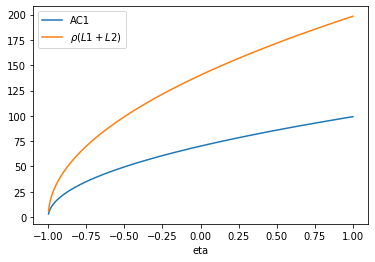
\includegraphics[scale=0.5]  {problem4.png}}        
 \caption{\label{2} risk allocation}      
 \end{figure}

Apparently, risk measure increases as correlation coefficient increases. It's reasonable since when two assets more correlated, there is less power to diverse the risk with only this two assets. Also, we can see the risk allocation also increases, however, the proportion doesn't change.

$$
\frac{AC_1}{\rho(L_1+L_2)} = \frac{Cov(L_1,L)}{\sqrt{Var(L)}\sqrt{Var(L)}} = \frac{1}{2}
$$

\begin{figure}[htbp]        
 \center{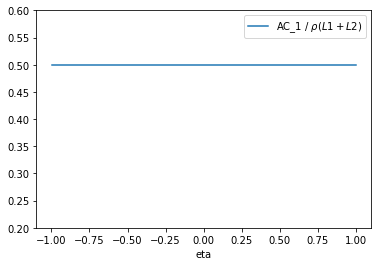
\includegraphics[scale=0.5]  {problem4.2.png}}        
 \caption{\label{2} risk allocation proportion}      
 \end{figure}

This is also reasonable since the distribution of two assets are the same and our $L = L_1 + L_2$, equally weighted. Thus the proportion of risk allocation shouldn't change.

The code is in Appendix.

\section*{Appendix}
\textbf{code for problem 1:}
\begin{lstlisting}[title=code for problem 1, frame=shadowbox]
import numpy as np
import math
import matplotlib.pyplot as plt

#problem 1(a)
N = 100
p = 0.991
mu = -50*0.991+1000*0.009
var = (-50-mu)**2 * p + (1000 - mu)**2 * (1-p)
alpha = [(i+1)/N for i in range(N)]
Ent = [mu+a*var/2 for a in alpha]

plt.plot(alpha,Ent)
plt.ylabel('Ent(L)')
plt.xlabel('alpha')
plt.show()

#problem 1(b)
alpha = [(i+1)/N for i in range(N)]
mu12 = -100 * (p**2) + 950 * 2*p*(1-p) + 2000 * (1-p)**2
var12 =  (-100 - mu12)**2 * (p**2) + (950 - mu12)**2 * 2*p*(1-p) + (2000 - mu12)**2 * (1-p)**2
Ent_b = [mu12+a*var12/2 for a in alpha]

plt.plot(alpha,Ent)
plt.ylabel('Ent(L1+L2)')
plt.xlabel('alpha')
plt.show()

#problem 1(c)
# here a is the probability of (-50,-50), and thus correspondingly we know
#P(-50,1000) = 1-p-a, P(1000,-50) = 1-p-a, P(1000,1000) = a+2p-1
p = 0.991
mu = -50*p+1000*(1-p)
var = (-50-mu)**2 * p + (1000-mu)**2 * (1-p)
N = 1000
alpha = 0.99

def compute_a(rho):
    RHS = mu**2 + rho*var
    RHS = RHS - (10**6 - (10**5 + 2 * 10**6)*p)
    a = RHS / (2500+10**5+10**6)
    
    return a

rho = [-1+2*i/N for i in range(N)]

Ent_c = []
SR_c = []
GLR_c = []
SOR_c = []
for r in rho:
    p1 = compute_a(r)
    p2 = 2*p - 2*p1
    p3 = 1 - 2*p + p1
#     print(p1,p2,p3,p1+p2+p3)
    mu_12 = -100*p1 + 950*p2 + 2000*p3
    var_12 = (-100 - mu_12)**2 * p1 + (950 - mu_12)**2 * p2 + (2000 - mu_12)**2 * p3
    mu_plus = 950*p2 + 2000*p3
    mu_plus_square = 950**2 * p2 + 2000**2 * p3
    Ent_c.append(mu_12+alpha*var_12/2)
    SR_c.append(- mu_12 / np.sqrt(var_12))
    GLR_c.append(- mu_12 / mu_plus)
    SOR_c.append(- mu_12 / np.sqrt(mu_plus_square))

plt.figure(figsize = (15,10))
ax1 = plt.subplot(2,2,1)
plt.title('Ent(L1+L2)')
ax2 = plt.subplot(2,2,2)
plt.title('SR(L1+L2)')
ax3 = plt.subplot(2,2,3)
plt.title('GLR(L1+L2)')
ax4 = plt.subplot(2,2,4)
plt.title('SOR(L1+L2)')

plt.sca(ax1)
plt.plot(rho,Ent_c)
plt.sca(ax2)
plt.plot(rho,SR_c)
plt.sca(ax3)
plt.plot(rho,GLR_c)
plt.sca(ax4)
plt.plot(rho,SOR_c)

plt.show()
\end{lstlisting}

\textbf{code for problem 4:}
\begin{lstlisting}[title=code for problem 4, frame=shadowbox]
# problem 4
p = 0.991
mu = -50*p+1000*(1-p)
N = 1000
var = (-50-mu)**2 * p + (1000-mu)**2 * (1-p)

eta = [-1+2*(i+1)/N for i in range(N)]

AC1 = []
AC2 = []
y = []
for r in eta:
    AC1.append((var * (1+r)) / np.sqrt(2*var + 2*r*var))
    AC2.append(AC1[-1])
    y.append(np.sqrt(2*var + 2*r*var))

plt.plot(eta,AC1,label = 'AC1')
plt.plot(eta,y,label = r'$\rho (L1+L2)$')
# plt.ylim(0.2, 0.6)
plt.xlabel('eta')
plt.legend(loc = 'best')
plt.show()
\end{lstlisting}

\end{spacing}
\end{document}